\documentclass{article}
\usepackage{graphicx}
\usepackage[utf8]{inputenc}
\usepackage{fullpage}
\usepackage{listings}
\usepackage{xcolor}
\usepackage{url}
\usepackage[linesnumbered,ruled,vlined]{algorithm2e}
\usepackage{enumitem}
\usepackage{amsmath}
\usepackage{amsfonts}
\usepackage{amssymb}

\parindent0in
\pagestyle{plain}
\thispagestyle{plain}

\newcommand{\assignment}{Homework 1}
\newcommand{\duedate}{July 19, 2019}

% traduzindo o nome das figuras
\renewcommand{\figurename}{Figura}

%QED Symbol
\newcommand*{\QEDA}{\hfill\ensuremath{\blacksquare}}%
\newcommand*{\QEDB}{\hfill\ensuremath{\square}}%


% \renewcommand\thesubsection{\arabic{subsection}}

\title{Homework 1}
\date{}

\begin{document}

Fundação Getulio Vargas\hfill\\
Estruturas de Dados e Algoritmos\hfill\textbf{\assignment}\\
Prof.\ Jorge Poco\hfill\textbf{Due:}: \duedate\\
\smallskip\hrule\bigskip

{\let\newpage\relax\maketitle}
\maketitle

\section{Induction [3pts]}
Answers should be written in this document. 

\begin{enumerate}
  \item Prove by Induction that:
  \( \sum_{i=1}^{n}i^2=\frac{n(n+1)(2n+1)}{6} \qquad\forall n \geq 0\)
    
    \textcolor{red}{Resposta: }
    \begin{enumerate}[itemsep=0pt, label=(\roman*)]
        \item Caso base: considere $n=1$. Então, 
        $\sum_{i=1}^{n} i^2= 1^2 = \frac{1(1+1)(2\cdot 1 + 1)}{6} = \frac{2 \cdot 3}{6} = \frac{6}{6}$
        o que é verdadeiro. Então, a proposição é válida para $n=1$. Tomemos agora o passo de indução. 
        
        \item Passo indutivo: Suponha que, para algum $n \in \mathbb{N}$, a seguinte proposição é verdadeira: 
        \begin{equation} \label{ind:1-hip-ind}
            \sum_{i=1}^{n}i^2 = \frac{n(n+1)(2n+1)}{6}
        \end{equation}
        Queremos mostrar que, dado que a proposição é válida para $n \in \mathbb{N}$, ela também será válida para $n+1 \in \mathbb{N}$, isto é, que 
        $$\sum_{i=1}^{n+1}i^2 = \frac{(n+1)\cdot [(n+1)+1]\cdot [2(n+1)+1])}{6} =\frac{(n+1)(n+2)(2n+3)}{6}$$. 
        
        Partindo da hipótese de indução, de \ref{ind:1-hip-ind}, temos:
        
        \begin{equation*}
            \sum_{i=1}^{n}i^2 + (n+1)^2 = \sum_{i=1}^{n+1}i^2= \frac{n(n+1)(2n+1)}{6} + (n+1)^2 = \frac{n(n+1)(2n+1) + 6(n+1)^2}{6} = 
        \end{equation*}
        
        \begin{equation*}
             = \frac{(n+1)}{6}\left[  n(2n+1) + 6(n+1)\right] = \frac{(n+1)}{6}\left[ 2n^2 + n + 6n + 6\right] = 
        \end{equation*}
        
        \begin{equation*}
            = \frac{(n+1)}{6}\left[  2n^2 + 7n + 6 \right] \\ = \frac{(n+1)}{6}\left[ (n+2)(2n+3) \right]
        \end{equation*}
        Como queríamos demonstrar. \QEDA
    \end{enumerate}
    
  \item Prove by Induction that:
  $\forall n \geq 7$ it is true $3^n<n!$
  
  \textcolor{red}{Resposta: }
    \begin{enumerate}[itemsep=0pt, label=(\roman*)]
    
    \item Caso base: Tome $n=7$. Assim, $3^7<7! \iff 2187 < 5040$, o que é verdade.
    
    \item Passo indutivo: Suponha, para um certo $n \in \mathbb{N}$, que $3^n <n!$. Então, multiplicando ambos os lados por $(n+1)$, temos:
    
    \begin{equation*}
        3^n (n+1) < n! \cdot (n+1) \Rightarrow{} n3^n + 3^n < (n+1)!
    \end{equation*}
    
    Como estamos tomando $n \geq 7$, sabemos que $n+1>3$. Portanto, 
    
    \begin{equation*}
        3^{n+1} < (n+1)\cdot 3^n < (n+1)!
    \end{equation*}
     \QEDA
    \end{enumerate}
  
  
  \item Prove by Induction that $\forall n \geq 0$
  \[
    \left \lceil\frac{n}{2} \right \rceil=
    \left\{
    \begin{array}{ll}
    \frac{n}{2}& \textrm{si $n$ es par}\\
    \frac{n+1}{2}& \textrm{si $n$ es impar}
    \end{array}
    \right.
  \]
  
    \textcolor{red}{Resposta: }
    \begin{enumerate}[itemsep=0pt, label=(\roman*)]
    
    \item Caso base: Considere $n=0$ (par) ou $n=1$ (ímpar). Então, 
    
    \begin{equation*}
        n=0 \Rightarrow{} \left\lceil \frac{n}{2} \right \rceil = \frac{0}{2} = 0
    \end{equation*}
    
    \begin{equation*}
        n=1 \Rightarrow{} \left \lceil \frac{n}{2} \right \rceil = \frac{1+1}{2} = 1
    \end{equation*}
    
    Logo, a proposição é verdadeira para o caso base.
    
    \item Passo indutivo: Suponha que, para algum $n \in \mathbb{N}$, é válido que:
    
    \[
    \left \lceil\frac{n}{2} \right \rceil=
    \left\{
    \begin{array}{ll}
    \frac{n}{2}& \textrm{se $n$ é par}\\
    \frac{n+1}{2}& \textrm{se $n$ é ímpar}
    \end{array}
    \right.
    \]
    
    Logo, se $n$ é par, $n+1$ é ímpar. Nesse caso, teremos: 
    
    \begin{equation}\label{ind:3-ind}
        n = 2m, m \in \mathbb{Z_{+}} \Rightarrow{} \left \lceil \frac{n+1}{2} \right \rceil = \left \lceil \frac{2m+1}{2}\right \rceil = \left \lceil m+\frac{1}{2}\right \rceil = m+1 = \frac{(2m+1)+1}{2} = \frac{(n+1)+1}{2}
    \end{equation}
    
    Agora, se $n$ é ímpar, então $n+1$ é par e temos:
    
    \begin{equation}\label{ind:3-ind}
        n = 2m+1, m \in \mathbb{Z_{+}} \Rightarrow{} \left \lceil \frac{n+1}{2} \right \rceil = \left \lceil \frac{2m+2}{2}\right \rceil = \left \lceil m+1\right \rceil = m+1 = \frac{(2m+1)}{2} = \frac{(n+1)}{2}
    \end{equation}
    
    Que é exatamente a proposição que queríamos demonstrar. \QEDA
    
    \end{enumerate}
  
  
  
    \item Prove by induction that a number is divisible by 3 if and only if the sum of its digits is divisible by 3.
    
    \textcolor{red}{Resposta: }
    \begin{enumerate}[itemsep=0pt, label=(\roman*)]
    
    \item Caso base:
    
    \item Passo indutivo:
    
    \end{enumerate}
    
    
    
    \item Prove that any integer greater than 59 can be formed using only 7 and 11 cent coins.
    
    \textcolor{red}{Resposta: }
    \begin{enumerate}[itemsep=0pt, label=(\roman*)]
    
    \item Caso base: Considere $n = 60$. Nesse caso, podemos escrever:
    
    \begin{equation*}
        60 = 7\cdot 7 + 1 \cdot 11
    \end{equation*}
    
    Assim, conseguimos 60 centavos se adicionarmos 7 moedas de 7 centavos a uma moeda de 11 centavos. Logo, a proposição é válida para $n=60$. 
    
    \item Passo indutivo: Suponha que, para $n \in \mathbb{N}$, a proposição é verdadeira. Isto é, $n = 7a + 11b$, com $a,b \in \mathbb{Z}_{+}$. 
    
    Assim, para $n+1$, temos: 
    
    \begin{equation*}
        n+1 = 7w+11z.
    \end{equation*}
    
    Tome $w = a-3$ e $z = b+2$. Assim, 
    
    \begin{equation*}
        7w+11z = 7(a-3)+11(b+2)=7a-21+11b+22 = 7a+11b+1 = n+1
    \end{equation*}
    
    \QEDA
    \end{enumerate}
    
  \item Prove by induction that $F_{n+k}=F_{k}F_{n+1}+F_{k-1}F_{n}$
    
    \textcolor{red}{Resposta: }
    
    \textbf{OBS:} Vamos considerar $F_1=F_2=1$, $F_3 = 2$ e $F_n = F_{n-1}+F_{n-2}$, onde $F_n$ é o $n$-ésimo termo da sequência de Fibonacci. 
    
    \begin{enumerate}[itemsep=0pt, label=(\roman*)]
    
    \item Caso base: Consideremos o caso em que $n=1$. Então, 
    
    \begin{equation*}
        F_{k+1}=F_{k}F_{2}+F_{k-1}F_{1} = F_k + F_{k-1}
    \end{equation*}
    
    Que é exatamente a expressão que define a sequência de Fibonacci. Logo, a proposição é verdadeira para o caso base. 
    
    \item Passo indutivo: Considere que, para um certo $n \in \mathbb{N}$, é válido que $F_{n+k}=F_{k}F_{n+1}+F_{k-1}F_{n}$ e também que $F_{n+k-1}=F_{k}F_{n}+F_{k-1}F_{n-1}$. Queremos mostrar que essa igualdade também é verdadeira para $n+1 \in \mathbb{N}$, isto é, $F_{n+1+k}=F_{k}F_{n+2}+F_{k-1}F_{n+1}$. 
    
    Ora, sabemos que 
    
    \begin{equation*}
        F_{n+k+1} = F_{n+k} + F_{n+k-1}
    \end{equation*}
    
    Pela hipótese de indução, podemos escrever: 
    
    \begin{equation*}
        F_{n+k+1} = F_{k}F_{n+1}+F_{k-1}F_{n} + F_{k}F_{n}+F_{k-1}F_{n-1} = F_k(F_{n+1} + F_n) + F_{k-1}(F_n + F_{n-1}) \Rightarrow{}
    \end{equation*}
    
    \begin{equation*}
         \Rightarrow{} F_{n+k+1}= F_kF_{n+2}+F_{k-1}F_n
    \end{equation*}
    
    \QEDA
    
    \end{enumerate}
  
  
  \item Prove by induction in $n$ that \(\sum_{m=0}^{n}{n \choose m}=2^n\)
  
    \textcolor{red}{Resposta: }
    
    \textbf{OBS:} Esse resultado é um caso particular do \textbf{teorema binomial}. Vamos prová-lo por indução e, em seguida, apondar o caso particular que foi pedido para provar nesse item. \newline
    
    \textbf{Teorema Binomial:} Para qualquer $n \in \mathbb{N}$, 
    $$
    (x+y)^{n}=\sum_{m=0}^{n}{n \choose m}x^{m} y^{n-m}
    $$
    
    Provemos esse teorema por indução.
    
    \begin{enumerate}[itemsep=0pt, label=(\roman*)]
    
    \item Caso base: para $n=1$, temos:
    
    \begin{equation*}
        (x+y)^{1}=x+y={1 \choose 0} x^{0} y^{1-0}+{1 \choose 1} x^{1} y^{1-1}=\sum_{m=0}^{1}{1 \choose m} x^{m} y^{1-m}
    \end{equation*}
    
    Tomando $x=y=1$, temos o seguinte resultado: 
    
        \begin{equation*}
        (1+1)^{1}=2={1 \choose 0} 1^{0} 1^{1-0}+{1 \choose 1} 1^{1} 1^{1-1}=\sum_{m=0}^{1}{1 \choose m}
    \end{equation*}
    
    Portanto, a proposição é válida para $n=1$. 
    
    
    \item Passo indutivo: Suponha que é verdade que 
    
    \begin{equation} \label{ind:7-hip-ind}
        (x+y)^{n}=\sum_{m=0}^{n}{n \choose m} x^{m} y^{n-m}
    \end{equation}
    
    Queremos mostrar que
    
    $$
    (x+y)^{n+1}=\sum_{m=0}^{n+1}{n+1 \choose m}x^{m} y^{n+1-m}
    $$
    
    Para isso, considere o termo $(x+y)^{n+1}$. Ora,
    
    \begin{equation*}
    (x+y)^{n+1}=(x+y)(x+y)^{n} = (x+y)\left[\sum_{m=0}^{n}{n \choose m} x^{m} y^{n-m}\right] = 
    \end{equation*}
    
    \begin{equation*}
        = \sum_{m=0}^{n}{n \choose m} x^{m+1} y^{n-m}+\sum_{m=0}^{n}{n \choose m} x^{m} y^{n-m+1} = 
    \end{equation*}
    
    \begin{equation*}
        = x^{n+1} + \sum_{m=0}^{n-1}{n \choose m} x^{n+1} y^{n-m}+\sum_{m=0}^{n}{n \choose m} x^{m} y^{n-m+1} = 
    \end{equation*}
    
    \begin{equation*}
        = x^{n+1} + \sum_{m=1}^{n}{n \choose m-1} x^{n} y^{n+1-m}+\sum_{m=0}^{n}{n \choose m} x^{m} y^{n-m+1} = 
    \end{equation*}
    
    \begin{equation*}
        = x^{n+1} +y^{n+1} + \sum_{m=1}^{n}{n \choose m-1} x^{n} y^{n+1-m}+\sum_{m=1}^{n}{n \choose m} x^{m} y^{n-m+1} = 
    \end{equation*}
    
    \begin{equation*}
        = x^{n+1} +y^{n+1} + \sum_{m=1}^{n} \left[{n \choose m-1} + {n \choose m}\right] (x^{m}y^{n-m+1}) = 
    \end{equation*}
    
    \begin{equation} \label{ind:7-ind}
        = x^{n+1} +y^{n+1} + \sum_{m=1}^{n} {n+1 \choose m} x^{m}y^{n-m+1} = \sum_{m=0}^{n+1} {n+1 \choose m} x^{m}y^{n-m+1}
    \end{equation}
    
    Com isso, provamos, por indução, o teorema binomial. Agora, fazendo $x=y=1$ na equação \ref{ind:7-ind}, temos o seguinte resultado: 
    
    \begin{equation*}
        2^{n+1} = \sum_{m=0}^{n+1} {n+1 \choose m} 1^{m}1^{n-m+1} = \sum_{m=0}^{n+1} {n+1 \choose m}
    \end{equation*}
    
    Logo, do teorema binomial, segue que $ 2^{n} = \sum_{m=0}^{n} {n \choose m}$, como queríamos demonstrar.
    
    \QEDA
    \end{enumerate}
  
  
  \item Prove by induction that a graph with $n$ vertices can have at most  $\frac{n(n-1)}{2}$ edges.
  
    \textcolor{red}{Resposta: }
    \begin{enumerate}[itemsep=0pt, label=(\roman*)]
    
    \item Caso base: $n=1$. Um grafo com apenas 1 vértice não tem nenhuma aresta. Além disso, 
    
    $$
    \frac{1(1-1)}{2} = 0
    $$
    
    Portanto, a sentença é válida para $n=1$. 
    
    \item Passo indutivo: Suponha que um grafo com $n$ vértices possui $\frac{n(n-1)}{2}$ vértices. Se adicionarmos um vértice, o número máximo de conexões que ele terá é $n$. Assim, o $n+1$-ésimo vértice terá, no máximo, $n$ conexões. Logo, 
    
    $$
    \frac{n(n-1)}{2}+n = \frac{n^2-n+2n}{2} = \frac{(n+1)n}{2}
    $$
    Que é, exatamente, o número máximo de arestas que um grafo com $n+1$ vértices pode ter. 
    
    Com isso, mostramos que a sentença é válida $\forall~n \in \mathbb{N}$. \QEDA
    \end{enumerate}
  
  
  \item Prove by induction that a complete binary tree\footnote{http://web.cecs.pdx.edu/~sheard/course/Cs163/Doc/FullvsComplete.html} with $n$ levels has $2^n-1$ vertices.
  
    \textcolor{red}{Resposta: }
    \begin{enumerate}[itemsep=0pt, label=(\roman*)]
    
    \item Caso base: Considere uma árvore binária com apenas 1 nível. Nesse caso, ela tem apenas 1 vértice. Além disso, $2^1-1=1$, que é exatamente o número de vértices de uma árvore binária com um só nível. Assim, provamos que a proposição é válida para $n=1$. 
    
    \item Passo indutivo: Suponha que uma árvore binária de decisão com $n$ níveis possui $2^n-1$ vértices. Se adicionarmos um nível à essa árvore, dado que cada vértice dá origem a dois novos vértices (uma vez que a árvore é binária), ao adicionarmos o $n+1$-ésimo nível à árvore, aumentamos o número de vértices em $2^n$. Ainda, $2^n-1+2^n=2\cdot 2^n-1 = 2^{n+1}-1$, que é exatamente o que queríamos provar. 
    
    \QEDA
    
    \end{enumerate}
  
  
  \item A polygon is convex if each pair of points in the polygon can be joined by a straight line that does not leave the polygon. Prove by induction in $n>3$ that the sum of the angles of a polygon of $n$ vertices is $180(n-2)$.
  
  
    \textcolor{red}{Resposta: }
    \begin{enumerate}[itemsep=0pt, label=(\roman*)]
    
    \item Caso base: Considere $n=4$, ou seja, um polígono com 4 lados. Sabemos que a soma dos seus ângulos é 360 (que é exatamente a soma dos ângulos de um quadrado). Ainda, $180(4-2) = 180 \cdot 2 = 360$. Portanto, a afirmativa é verdadeira para $n=4$. 
    
    \item Passo indutivo: Agora, suponha que a soma dos ângulos internos de um polígono com $n$ lados, $n \in \mathbb{N}$, é exatamente $180(n-2)$. Queremos mostrar que a soma dos ângulos internos de um polígono com $n+1$ lados é $180(n+1-2) = 180(n-1)$
    
    Note que um polígono com $n$ lados pode ser seccionado em $n-2$ triângulos, como mostra a figura a seguir:
    
    \begin{figure}[!h]
        \centering
            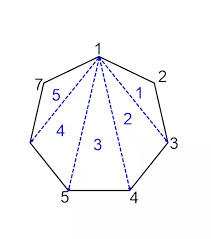
\includegraphics[scale=0.6]{Figures/hw1-img.png}
            \caption{Polígono de 7 lados subdividido em 5 triângulos}
        \label{fig:my_label}
    \end{figure}
    
    Sabemos que a soma dos ângulos internos de um triângulo é $180$ graus. Note que, se adicionamos mais um lado a um polígono de $n$ lados, conseguimos formar mais um triângulo em seu interior. Assim, adicionamos $180$ graus à soma dos seus ângulos internos. Em outras palavras, a soma dos ângulos internos de um polígono com $n+1$ lados será: 
    $$
    180(n-2) + 180 = 180\left [1+(n-2) \right] = 180(n-1)
    $$
    
    Que é exatamente o que queríamos demonstrar. \QEDA
    
    \end{enumerate}
  
\end{enumerate}

\section{Correctness of bubblesort [2pts]}
Bubblesort is a popular, but inefficient, sorting algorithm. It works by repeatedly swapping adjacent elements that are out of order.

\begin{algorithm}[H]
\SetAlgoLined
  \For{$i = 1$ \textbf{to} $A.length -1$} {
    \For{$j = A.length$ \textbf{downto} $i + 1$} {
      \If{$A[j] < A[j-1]$} {
        exchange $A[j]$ with $A[j-1]$
      }
    }
  }
\caption{BUBBLESORT(A)}
\end{algorithm}

\begin{enumerate}[label=\Alph*]
  \item Let $A'$ denote the output of BUBBLESORT(A). To prove that BUBBLESORT is correct, we need to prove that it terminates and that
  
  \begin{equation} \label{eq:1}
    A'[1] \leq A'[2] \leq ... \leq A'[n]
  \end{equation}
  
  where $n = A.length$. In order to show that BUBBLESORT actually sorts, what else do we need to prove?
  
  \vspace{2cm} 
  \textcolor{red}{Resposta:}
  
  Além do que foi mencionado, precisamos mostrar que os elementos da lista ordenada \textit{A'} e da lista inicial \textit{A} são os mesmos, mas não necessariamente na mesma ordem. 
  
  \vspace{\baselineskip}
  The next two parts will prove inequality~(\ref{eq:1}).
  
  \item State precisely a loop invariant for the \textbf{for} loop in lines 2–6, and prove that this loop invariant holds. Your proof should use the structure of the loop invariant proof presented in this chapter.
  
  \textcolor{red}{Resposta:}
  
  Para provar que o \textit{loop} de um algoritmo cumpre seu objetivo, devemos mostrar que a condição invariante analisada no \textit{loop} é verdadeira em cada uma das seguintes etapas:
  
  \begin{itemize}
      \item \textbf{Inicialização:} a condição é verdadeira antes da primeira iteração do \textit{loop}.
      
      \item \textbf{Manutenção:} a condição é verdadeira antes da $n$-ésima iteração do \textit{loop} e também é verdadeira antes da $(n+1)$-ésima iteração (ao fim da $n$-ésima).  
      
      \item \textbf{Finalização:} ao fim da última iteração do \textit{loop}, o invariante permanece verdadeiro.
  \end{itemize}
  
  O invariante é uma propriedade que permanece verdadeira em cada uma das etapas e ajuda a analisar se o algoritmo cumpre apropriadamente o seu objetivo (está correto).
  
  No caso do \textbf{loop das linhas 2-6}, podemos destacar a seguinte propriedade: 
  \begin{center}
      \textbf{P1:} A cada iteração, o elemento $\normalfont{A}[j]$ é o menor elemento da lista $\normalfont{A}[j,\dots, \normalfont{A}.length]$
  \end{center}
  
  Vamos provar que essa propriedade se cumpre em cada uma das etapas citadas acima. 
  
  \begin{itemize}
      \item Inicialização: Como $j = A.length$, temos que a lista $\normalfont{A}[j, \dots , \normalfont{A}.length] = A[j]$. Logo, trivialmente, $\normalfont{A}[j]$ é seu maior elemento.
      
      \item Manutenção: A cada iteração, se $\normalfont{A}[j-1]<\normalfont{A}[j]$, os termos são trocados. Assim, na lista alterada, $\normalfont{A}[j-1,j]$, $\normalfont{A}[j-1]$ é o menor dos dois elementos. Assim, a lista $\normalfont{A}[j-1,\dots,\normalfont{A}.length]$ sempre terá $\normalfont{A}[j-1]$ como menor elemento.
      
      \item Finalização: Quando $j=i+1$, temos que o elemento $\normalfont{A}[i]=\normalfont{A}[j-1]$ será o menor elemento da lista $\normalfont{A}[i,\dots,\normalfont{A}.length]$
  \end{itemize}
  
    Com isso, provamos que a propriedade \textbf{P1} permanece verdadeira em cada uma das etapas. Logo, $P1$ é o invariante do \textit{loop} das linhas 2-6.
  
  
  
  \item Using the termination condition of the loop invariant proved in part (B), state a loop invariant for the for loop in lines 1–7 that will allow you to prove inequality~(\ref{eq:1}). Your proof should use the structure of the loop invariant proof presented in this chapter.
  
  Vamos mostrar que a propriedade \textbf{P2} abaixo é o invariante do \textbf{\textit{loop} externo das linhas 1-7}.
  
  \textcolor{red}{Resposta: }
  
  \begin{center}
      \textbf{P2:} A lista $\normalfont{A}[1,\dots,j]$ está ordenada, i.e., $\normalfont{A}[1] \leq \normalfont{A}[k] \leq \normalfont{A}[j],~\forall~k=1,\dots,j.$
  \end{center}
  
  \begin{itemize}
      \item Inicialização: Antes da primeira iteração, quando $i=1$, temos $\normalfont{A}[1,\dots,i] = \normalfont{A}[1]$. Portanto, a lista está trivialmente em ordem crescente.
      
      \item Manutenção: Como resultado do \textit{loop} interno (das linhas 2-6), a lista $\normalfont{A}[i,\dots,\normalfont{A}.length]$ tem $\normalfont{A}[i]$ como menor elemento. Assim, $\normalfont{A}[i]\leq A[j],~\forall~j=i+1,\dots,A.length$.
      
      \item Finalização: Quando $i=A.length$, temos como resultado uma lista $A[1,\dots,i,\dots,A.length]$ ordenada.
      
  \end{itemize}
 
  
  \item What is the worst-case running time of BUBBLESORT? How does it compare to the running time of insertion sort?
  
  \textcolor{red}{Resposta:}
  
  A tabela abaixo exibe o número de comparações feitas pelo Bubble Sort para o $j$-ésimo elemento, com $j=1,\dots,n$, onde $n$ é o tamanho do vetor.
  
  \begin{center}
      \begin{tabular}{c|c}
           \textbf{Elemento}&\textbf{\# de Comparações}  \\
           \hline
           $1$ & $(n-1)$ \\
           $2$ & $(n-2)$ \\
           \vdots & \vdots \\
           $j$ & $(n-j)$ \\
           \vdots & \vdots \\
           $(n-1)$ & $1$ \\ 
      \end{tabular}
  \end{center}
\end{enumerate}

Assim, a complexidade do Bubble Sort é dada por:

$$
(n-1)+(n-2)+\dots+1 = \frac{n(n-1)}{2} = \frac{n^2-n)}{2}, \text{ i.e., } O(n^2)
$$

Que é exatamente a complexidade do algoritmo Insertion Sort no pior cenário (quando o vetor está ordenado em ordem decrescente). 

No melhor caso, i.e., quando os elementos do vetor já estão em ordem crescente, a complexidade de tempo do Insertion Sort é $O(n)$, enquanto que o Bubble Sort continua tendo complexidade $O(n)$. 

\vspace{\baselineskip}

\textbf{OBS:} Dizemos que a complexidade do Bubble Sort é $\Theta(n)$.



\section{Growth of Functions [2pts]}

\begin{enumerate}[label=\Alph*]
  \item For each of the following pairs of functions, either $f(n)$ is in $O(g(n))$, $f(n)$ is in $\Omega(g(n))$, or $f(n) = \Theta(g(n))$. Determine which relationship is correct and briefly explain why.
  
  \textbf{Definições:}
  \begin{enumerate}[itemsep=0cm,label=(\alph*)]
      \item $ f(n)=O(g(n))$ se $\exists~N \in \mathbb{N}, \text{ e } \exists~c \in \mathbb{R}_+$ tal que, $\forall~n \in \mathrm{N}$, se $n \geq N$, então $ f(n) \leq c \cdot g(n)$.
      
      \item $f(n)=\Omega(g(n))$ se $\exists~N \in \mathbb{N} \text{ e } \exists~c \in \mathbb{R}_+$ tal que, $\forall~n \in \mathbb{N}$, se $n \geq N$, então $f(n) \geq c\cdot g(n)$.
      
      \item $f(n)=\Theta(g(n))$ se (a) e (b) são satisfeitas, isto é, $f(n)=O(n)$ e $f(n)=\Omega(g(n))$
  \end{enumerate}
  
    \begin{itemize}
      \item $f(n) = \log n^2$; $g(n) = \log n + 5$
      
      \textcolor{red}{Resposta: } 
      
      Vamos verificar quais definições, (a), (b) ou (c) são satisfeitas.
      
      \begin{enumerate}[itemsep=0cm, label=(\alph*)]
          \item $f(n)=O(g(n))$. Para ver isso, tome $N=1$ e $c=3$. Assim, 
          $f(n)=2 \log n \leq 3 \log n+15=c g(n)$. 
          
          \item Faça $c=1$ e $N=32,$ temos $f(n)=2 \log n \geq \log n+5=c g(n)$. Assim, é fácil ver que $f(n)=\Omega(g(n))$.
          
          \item Note que, de (a) e (b), temos que $\mathrm{f}(\mathrm{n})=\mathrm{O}(\mathrm{n})$ e $\mathrm{f}(\mathrm{n})=\Omega(g(n))$. Logo, $f(n)=\Theta(g(n))$.
      \end{enumerate}
      
      \item $f(n) = \log^2 n$; $g(n) = \log n$
      
      \textcolor{red}{Resposta: } 
      
      \begin{enumerate}[itemsep=0cm, label=(\alph*)]
          \item $\not \exists~c \in \mathbb{R}_+,~N \in \mathbb{N}$ tais que $f(n) \leq c\cdot g(n)$, se $n \geq N$. Logo, $f(n)\not =O(g(n))$.
          
          \item Faça $c=1$ e  $N=4$. Assim, temos $f(n)=\log n \cdot \log n=4 \geq 2=\log n=c \cdot g(n)$. Logo, $f(n)=\Omega(g(n))$.
          
          \item Como a definição (a) não é satisfeita, temos apenas que $f(n)=\Omega(g(n))$. 
      \end{enumerate}
      
      
      \item $f(n) = n\log n + n$; $g(n) = \log n$
      
      \textcolor{red}{Resposta: } 
      
      \begin{enumerate}[itemsep=0cm, label=(\alph*)]
          \item $\not \exists~c \in \mathbb{R}_+,~N \in \mathbb{N}$ tais que $f(n) \leq c\cdot g(n)$, se $n \geq N$. Logo, $f(n)\not =O(g(n))$.
          
          \item Escolha $c=1$ e $N=2$. Assim, $f(n)=n \cdot \log n \cdot \log n=4 \geq 1 =1 \cdot \log n=c \cdot g(n)$. Portanto, $f(n)=\Omega(g(n))$.
          
          \item Como apenas a definição (a) é satisfeita, podemos afirmar apenas que $f(n)=\Omega(g(n))$. 
      \end{enumerate}

      \item $f(n) = 2^n$; $g(n) = 10n^2$
      
      \textcolor{red}{Resposta: } 
      
      \begin{enumerate}[itemsep=0cm, label=(\alph*)]
          \item $\not \exists~c \in \mathbb{R}_+,~N \in \mathbb{N}$ tais que $f(n) \leq c\cdot g(n)$, se $n \geq N$. Logo, $f(n)\not =O(g(n))$.
         
          \item Escolhendo convenientemente $c=\frac{1}{10}$ e $N=5$, temos: $f(n)=2^{n}=32 \geq 25=n^{2}=c g(n)$. Assim, $f(n)=\Omega(g(n))$. 
          
          \item Somente a definição (a) é satisfeita. Logo, temos que $f(n)=\Omega(g(n))$. 
      \end{enumerate}
    \end{itemize}
  
  \vspace{\baselineskip}
  \item Prove that $n^3 -3n^2 -n+1 = \Theta(n^3)$.
  
  \textcolor{red}{Resposta: } 
  
    \begin{enumerate}[itemsep=0cm, label=(\alph*)]
      \item Tome $c=6$ e $N=1$. Assim, $n^{3}-3 n^{2}-n+1 \leq n^{3}+3 n^{3}+n^{3}+n^{3}=6 n^{3}$. Logo, $f(n) =O(g(n))$.
      
      \item Escolha $c=\frac{1}{10}$ e $N=5$. Assim, $5^{3}-3 \cdot 5^{2}-5+1=46 \geq \frac{5^{3}}{10} = 12,5$. Portanto, $f(n)=\Omega(g(n))$.
      
      \item Como as definições (a) e (b) são satisfeitas, afirmamos que $f(n)=\Theta(g(n))$. 
    \end{enumerate} \QEDA
    
  \item Prove that $n^2 = O(2^n)$.

  \textcolor{red}{Resposta: } 
  
    Ora, $n^2<2^n,~\forall~n > 4$. Além disso, não existem $c \in \mathbb{R}_+$ e $N \in \mathbb{N}$ tais que, se $n \geq N$,  $ n^{2}>c \cdot 2^{n}$, isto é, $n^2 \not = \Omega(2^n)$
    
    Portanto, $n^2 = O(2^n)$. \QEDA
  
\end{enumerate}


\section{Insertion Sort - Mergesort - Quicksort [3pts]}
Implement the insertion sort, merge sort and quicksort using the template \texttt{test.py} (use Python 3.X). Create a \texttt{test.cpp} file and write the equivalent code from \texttt{test.py} in C++, ie., the functions: main, \texttt{insertion\_sort}, \texttt{merge\_sort}, \texttt{quicksort} and \texttt{is\_sorted}. For the random number generations you can use the \texttt{rand} function from \texttt{cstdlib}\footnote{\url{http://www.cplusplus.com/reference/cstdlib/rand/}}. Your code should print the tuple (number of objects, time insertion\_sort, time merge\_sort, time quicksort)

You must submit both \texttt{test.py} and \texttt{test.cpp}. Graphs and descriptions must be included in this document. 

\subsection{Random Order}
\begin{enumerate}
  \item Create 10 sets of numbers in random order. The sets must have \{10k, 20k, 30k, ..., 100k\} numbers.
  
  \item Sort these numbers using the 3 algorithms and calculate the time each algorithm takes for each set of numbers.
  
  \item Generate a plot (using excel or another tool) showing a \emph{linechart}, where the $x$-axis is the ``number of elements", and the $y$-axis is the time that the algorithms took in C++ and Python. This plot must have 6 lines of different colors with a legend.
  
  \item Write a small paragraph (3 to 4 lines) describing the results.
  
  \textcolor{red}{Resposta:}
  
  A figura abaixo exibe os tempos de execução de cada algoritmo (Insertion Sort, Merge Sort e Quicksort), no caso em que os vetores têm elementos aleatórios. 
  
  \begin{figure}[!h]
    \centering
    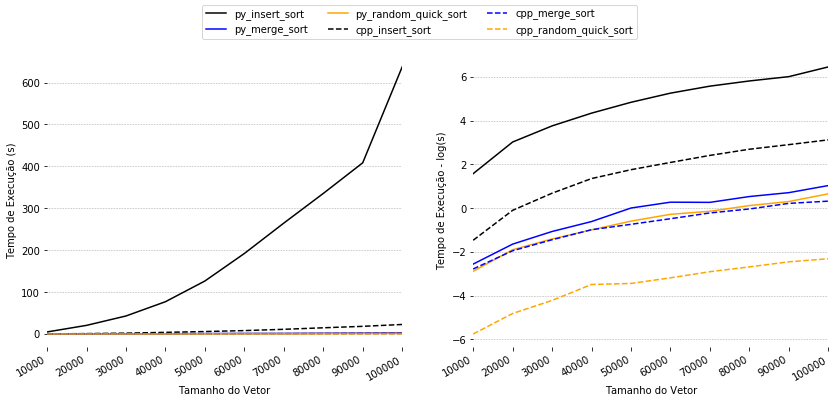
\includegraphics[scale=0.5]{Figures/random.png}
    \caption{Tempo de execução com vetores em ordem aleatória}
    \label{fig:graf-random}
  \end{figure}
\end{enumerate}
    
    Nesse gráfico, podemos destacar dois pontos:
    
    \begin{enumerate}
        \item O Insertion Sort foi o algoritmo mais ineficiente dos três testados (o que apresentou o maior tempo de execução). Isso já era esperado dado que a complexidade desse algoritmo é dada por $O(n^2)$, no pior caso, enquanto que o Merge Sort $O(n \cdot log n)$ $O(n^2)$. Já o Quicksort, devido à sua natureza aleatória, tem complexidade $C(n)$ tal que $O(n \cdot log n) \leq C(n) \leq O(n^2)$. Assim, à medida que aumentamos o tamanho do vetor, é esperado que o tempo gasto pelo Insertion Sort aumente na ordem de $n^2$, isto é, mais rápido que para os demais algoritmos. 
        
        \item Para todos os três algoritmos testados, o tempo de execução apresentado pelo C++ foi inferior ao tempo de execução do Python, o que reflete o fato de C++ ser uma linguagem compilada, enquanto o Python é uma linguagem interpretada (executada linha a linha). 
    \end{enumerate}

\subsection{Ascending Order}
Do the same experiment when the numbers are ordered in ascending order.

\vspace{\baselineskip} 
\textcolor{red}{Resposta:}

  A figura abaixo exibe os tempos de execução de cada algoritmo, no caso em que os vetores estão ordenados de maneira crescente (o que seria o melhor dos casos).  
\begin{figure}[!h]
    \centering
    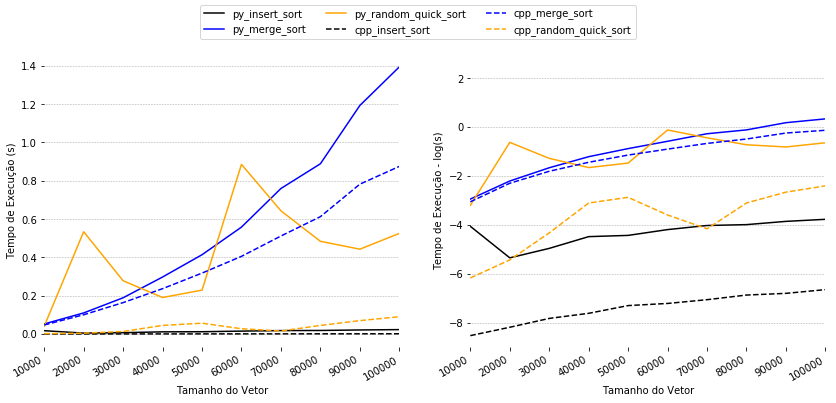
\includegraphics[scale=0.5]{Figures/ascending.png}
    \caption{Tempo de execução com vetores em ordem crescente (melhor caso)}
    \label{fig:graf-random}
\end{figure}

    
    Nesse gráfico vemos que o algoritmo Merge Sort foi o pior dos três (gastou mais tempo em execução), uma vez que sua complexidade é dada por $O(n \cdot log n)$. Assim, no caso em que os vetores já estão ordenados, o Insetion Sort e o Quick Sort são mais rápidos, dado que suas complexidades são $O(n)$ e $C(n)$, com $O(n) \leq C(n) \leq O(n \cdot log n)$. 
        

\subsection{Descending Order}
Do the same experiment when the numbers are ordered in descending order.

\vspace{\baselineskip}

\textcolor{red}{Resposta:}

  A figura abaixo exibe os tempos de execução de cada algoritmo, no caso em que os vetores estão ordenados de maneira decrescente (o que configura o pior dos casos).  

\begin{figure}[!h]
    \centering
    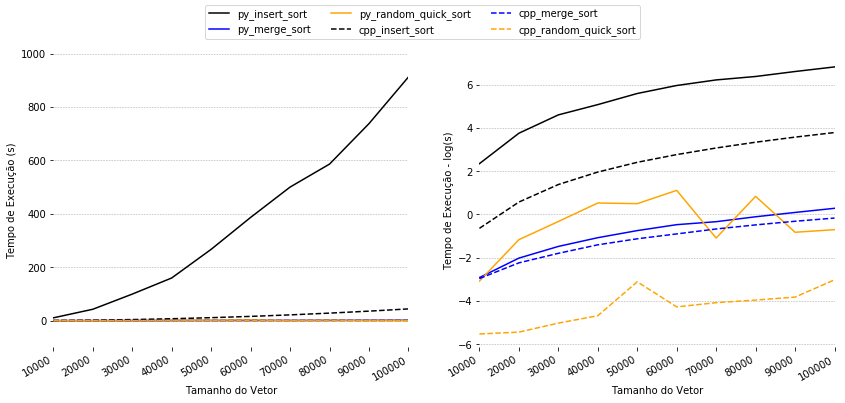
\includegraphics[scale=0.5]{Figures/descending.png}
    \caption{Tempo de execução com vetores em ordem decrescente (pior caso)}
    \label{fig:graf-random}
\end{figure}

    No gráfico acima, vemos que, no pior caso, o tempo de execução do Insertion Sort aumenta na ordem $O(n^2)$, o que é bem superior ao tempo gasto pelos outros dois algoritmos, que crescem (no máximo), na ordem $O(n \cdot log n)$

\end{document}